\chapter{Introdução}

\section{Delimitação do tema}

Modelos de Linguagem de Grande Escala, ou LLMs, são sistemas capazes de ler e produzir textos. Eles costumam responder de forma fluida e convincente, mas uma explicação bem escrita não garante que o raciocínio apresentado esteja correto. Esta pesquisa investiga essa diferença em uma tarefa simples de conferir: encontrar e explicar uma única jogada de Sudoku.

O Sudoku foi escolhido porque suas regras são objetivas. Uma pessoa ou um programa pode verificar se uma jogada respeita a linha, a coluna e o bloco da célula. Isso permite observar duas coisas separadamente: se a LLM chegou ao valor certo e se a explicação que ela deu realmente justifica esse valor.

O estudo trabalha com Sudokus 4 $\times$ 4 e 9 $\times$ 9. O tabuleiro começa com algumas células preenchidas, chamadas pistas, e outras vazias. O objetivo é preencher as células vazias sem alterar as pistas. Em cada linha, coluna e bloco, cada número permitido deve aparecer uma única vez. No Sudoku 4 $\times$ 4, usam-se os números de 1 a 4 e os blocos têm 2 $\times$ 2 células. No Sudoku 9 $\times$ 9, usam-se os números de 1 a 9 e os blocos têm 3 $\times$ 3 células.

\begin{figure}[!ht]
\centering
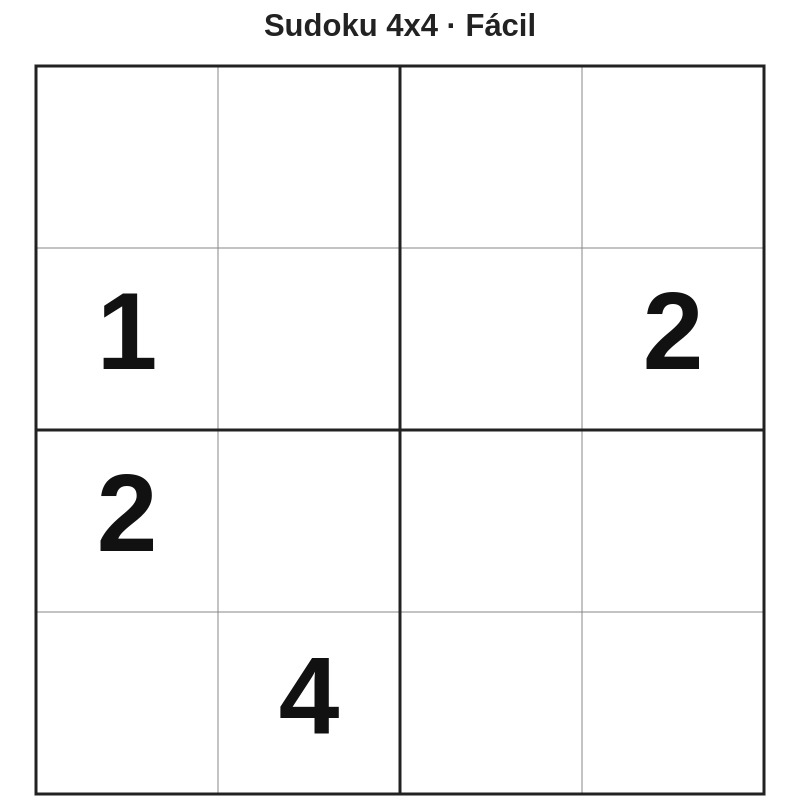
\includegraphics[width=0.62\textwidth]{figuras/sudoku-4x4-easy}
\Caption{Exemplo de tabuleiro Sudoku 4 $\times$ 4\label{fig:intro-sudoku}}
\Fonte{EducColorir (s.d.). Disponível em: \url{https://www.educolorir.com/gerador-de-sudoku}. Acesso em: 21 out. 2026.}
\end{figure}

Para indicar uma posição, o texto usa a forma L$\mathit{x}$C$\mathit{y}$, em que L significa linha e C significa coluna. A contagem começa em 1. Assim, L1C4 é a célula da primeira linha e da quarta coluna. Essa é uma notação pensada para leitura humana; mais adiante, a metodologia mostra como a mesma posição aparece no programa.

Uma célula vazia pode receber apenas números que não estejam em sua linha, coluna ou bloco. Esses números possíveis são chamados de candidatos. Se, em um Sudoku 4 $\times$ 4, uma célula não pode receber 1, 2 ou 4, resta apenas o número 3. A partir dessa ideia, a pesquisa analisa três maneiras de encontrar uma jogada.

No \textit{Naked Single}, uma célula fica com apenas um candidato. No \textit{Hidden Single}, um número pode continuar sendo candidato em mais de uma célula do tabuleiro, mas só pode aparecer em uma posição de uma linha, coluna ou bloco. No consenso de primeira camada, o programa considera hipóteses temporárias, acompanha o que acontece em cada uma e procura uma conclusão que se repete em todos os caminhos possíveis.

O recorte do estudo é uma jogada por vez e somente essas três técnicas. A intenção não é afirmar como uma LLM funciona internamente. O objetivo é verificar se ela produz uma jogada válida e se a explicação apresentada combina com a técnica solicitada.

\section{Problematização}

Quando uma LLM apresenta uma resposta convincente, é fácil assumir que ela raciocinou corretamente. Em tarefas lógicas, porém, ela pode acertar o valor por outro caminho, usar uma técnica diferente da pedida ou escrever uma justificativa que não sustenta a conclusão. Avaliar apenas a resposta final deixa esses casos escondidos.

O Sudoku cria um ambiente controlado para observar esse problema. As regras são claras, a jogada pode ser conferida automaticamente e a dificuldade pode ser ajustada. As técnicas de \textit{Naked Single} e \textit{Hidden Single} dependem apenas das informações visíveis no tabuleiro. O consenso exige que a LLM acompanhe hipóteses e compare as consequências de cada uma.

Diante disso, a pesquisa busca responder: como as LLMs se comportam ao indicar e justificar uma jogada de Sudoku que exige uma dedução direta ou uma comparação entre hipóteses?

\section{Hipótese}

Espera-se que as LLMs tenham melhor desempenho em \textit{Naked Single} e \textit{Hidden Single}, pois essas técnicas dependem de restrições visíveis na grade. No consenso, espera-se mais dificuldade, porque a tarefa exige manter hipóteses temporárias, acompanhar suas consequências e encontrar uma conclusão comum.

\section{Justificativa}

Avaliar LLMs com Sudoku ajuda a separar duas coisas que frequentemente aparecem misturadas: acertar uma resposta e explicar bem por que ela está certa. Como cada jogada pode ser conferida por regras objetivas, o estudo permite identificar respostas corretas com justificativas fracas, justificativas coerentes que chegam a uma conclusão errada e respostas que seguem exatamente a técnica solicitada.

Os resultados podem contribuir para avaliações de sistemas que precisam explicar suas decisões em linguagem clara. O estudo também oferece um conjunto de critérios simples para examinar respostas de LLMs em tarefas estruturadas, nas quais é possível conferir tanto o resultado quanto o caminho usado para chegar a ele.
